\section{Atividade 1}
\subsection{Descrição do Modelo}
O sistema modelado é um oscilador massa-mola-amortecedor, onde a massa está sujeita à força restauradora de uma mola e ao amortecimento proporcional à velocidade. A equação diferencial que descreve o movimento do sistema é dada por:
\[
m \ddot{x} + C \dot{x} + kx = 0
\]
onde \( x \) representa o deslocamento da massa \( m \) da sua posição de equilíbrio, \( \dot{x} \) é a velocidade, \( \ddot{x} \) é a aceleração, \( C \) é o coeficiente de amortecimento, e \( k \) é a constante da mola. A força de entrada é considerada nula, indicando que não há forças externas atuando sobre o sistema após o instante inicial.

\subsection{Parâmetros do Sistema}
Os parâmetros utilizados no modelo do sistema são especificados como segue:
\begin{itemize}
    \item Massa (\( m \)): 10 kg
    \item Coeficiente de amortecimento (\( C \)): 7 Ns/m
    \item Constante da mola (\( k \)): 5 N/m
\end{itemize}

As condições iniciais para a simulação, baseadas nos parâmetros acima, são detalhadas na tabela a seguir:
\begin{center}
\begin{tabular}{|c|c|c|}
\hline
\textbf{Caso} & \textbf{Velocidade Inicial \( V_0 \)} & \textbf{Posição Inicial \( X_0 \)} \\
\hline
1 & \( 5 \, \text{m/s} \) (\( \frac{m}{2} \)) & \( 0 \, \text{m} \) \\
2 & \( 0 \, \text{m/s} \) & \( 2.5 \, \text{m} \) (\( \frac{m}{4} \)) \\
3 & \( 3.33 \, \text{m/s} \) (\( \frac{m}{3} \)) & \( 2 \, \text{m} \) (\( \frac{m}{5} \)) \\
\hline
\end{tabular}
\end{center}

Esta tabela reflete os valores numéricos para cada caso, facilitando a compreensão e a aplicação direta dos parâmetros na simulação.

\subsection{Análise dos Resultados}
Cada um dos casos de simulação foi configurado com condições iniciais distintas para explorar como o sistema responde a diferentes estados iniciais de deslocamento e velocidade.

\subsubsection{Caso 1}
\begin{figure}[H]
    \centering
    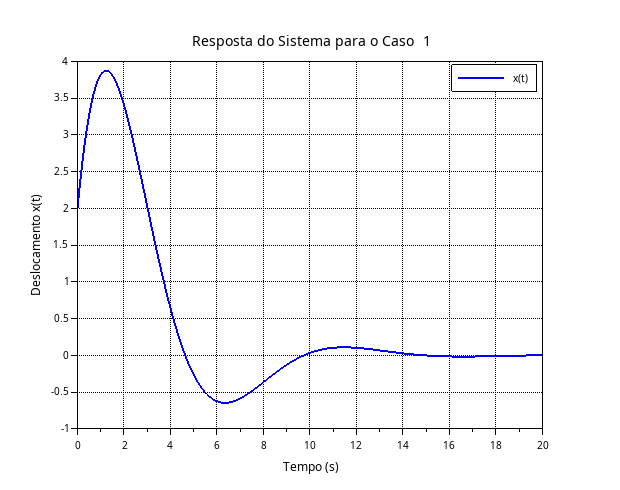
\includegraphics[width=0.7\textwidth]{1-atividade/assets/caso1.png}
    \caption{Resposta do sistema para o Caso 1}
\end{figure}
No Caso 1, com uma velocidade inicial significativa (\( \frac{m}{2} \)) e sem deslocamento inicial (\( X_0 = 0 \)), o sistema exibe uma resposta vigorosa inicialmente, decaindo rapidamente devido ao amortecimento considerável. A alta velocidade inicial resulta em uma amplitude inicial grande, mas a ausência de força externa e o alto amortecimento fazem com que o sistema retorne rapidamente à estabilidade sem oscilações residuais.

\subsubsection{Caso 2}
\begin{figure}[H]
    \centering
    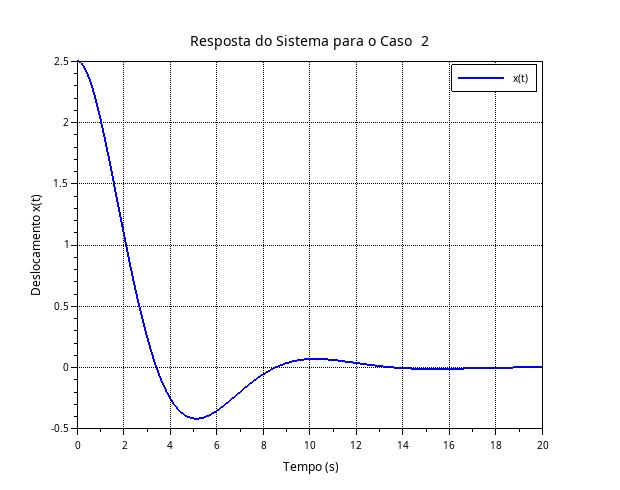
\includegraphics[width=0.7\textwidth]{1-atividade/assets/caso2.png}
    \caption{Resposta do sistema para o Caso 2}
\end{figure}
No Caso 2, a velocidade inicial é nula (\( V_0 = 0 \)), e o deslocamento inicial é \( \frac{m}{4} \). Este caso ilustra um exemplo clássico de oscilação amortecida onde o sistema é deslocado de sua posição de equilíbrio e liberado. A resposta mostra oscilações que decaem ao longo do tempo, com o sistema eventualmente retornando ao repouso. Comparativamente, este caso tem uma resposta mais suave em termos de velocidade devido à ausência de velocidade inicial.

\subsubsection{Caso 3}
\begin{figure}[H]
    \centering
    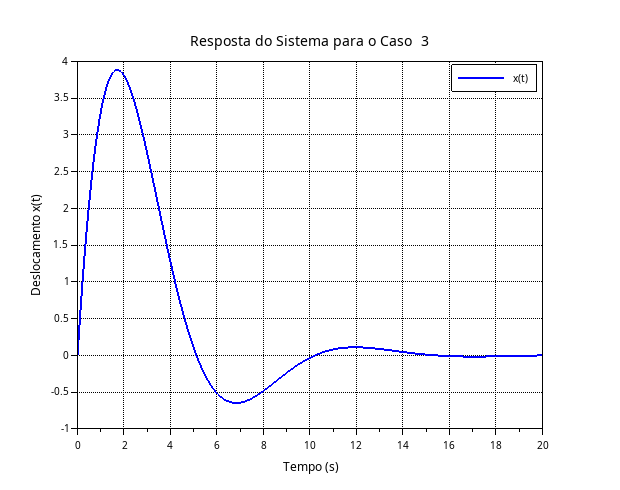
\includegraphics[width=0.7\textwidth]{1-atividade/assets/caso3.png}
    \caption{Resposta do sistema para o Caso 3}
\end{figure}
No Caso 3, tanto a velocidade (\( \frac{m}{3} \)) quanto o deslocamento (\( \frac{m}{5} \)) iniciais são não nulos. Esta condição inicial resulta em uma resposta dinâmica complexa, com o sistema exibindo uma amplitude inicial maior e oscilações mais sustentadas comparadas aos outros casos. O sistema ainda retorna ao repouso, mas a trajetória é mais envolvente e ilustra a interação entre energia cinética e potencial no sistema.

\subsubsection{Comparação Unificada dos Casos}
\begin{figure}[H]
    \centering
    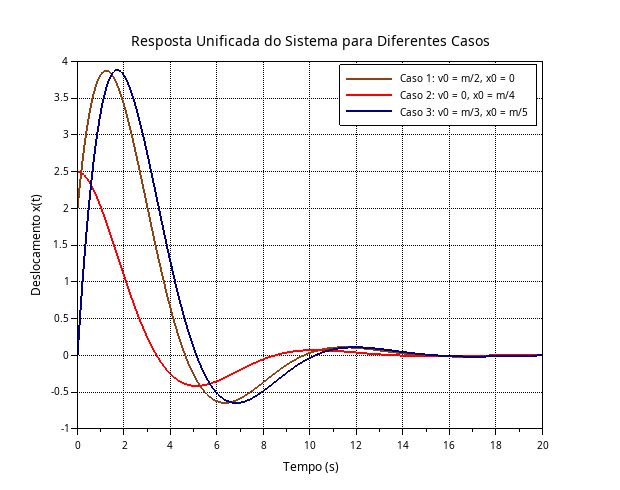
\includegraphics[width=0.7\textwidth]{1-atividade/assets/caso-all-in-one.png}
    \caption{Resposta unificada do sistema para os Casos 1, 2 e 3}
\end{figure}
A resposta unificada ilustra claramente as interações e diferenças nas dinâmicas do sistema sob diversas condições iniciais. Observando o gráfico, podemos notar que:
\begin{itemize}
    \item O \textbf{Caso 1} (Azul Escuro), com alta velocidade inicial e sem deslocamento, mostra a resposta mais rápida e com maior amplitude inicial, indicando uma rápida transferência de energia cinética para energia potencial e vice-versa, resultando em um rápido retorno à estabilidade.
    \item O \textbf{Caso 2} (Vermelho), começando com um deslocamento inicial sem velocidade, apresenta uma oscilação amortecida clássica que decai gradualmente, refletindo uma conversão mais lenta de energia potencial em energia cinética.
    \item O \textbf{Caso 3} (Marrom), com condições iniciais de deslocamento e velocidade moderados, combina aspectos dos dois primeiros casos, resultando em uma resposta intermediária com oscilações sustentadas que decaem de forma mais gradual que no Caso 1, mas com uma amplitude inicial mais significativa do que no Caso 2.
\end{itemize}
Esta comparação visual ressalta a importância do amortecimento e da rigidez da mola no comportamento do sistema, assim como o efeito das condições iniciais na resposta do sistema. Cada caso contribui para um entendimento mais aprofundado de como diferentes tipos de energia são gerenciados e dissipados dentro do sistema.


\subsection{Comentários Gerais}
Os gráficos mostram claramente a influência das condições iniciais na resposta dinâmica do sistema. A comparação entre os três casos revela que quanto maior a energia inicial (seja em forma de deslocamento ou velocidade), mais vigorosa é a resposta inicial do sistema. O amortecimento desempenha um papel crucial em trazer o sistema de volta ao repouso, demonstrando sua eficácia em dissipar energia mecânica. Essas simulações servem como uma excelente demonstração das propriedades fundamentais de sistemas dinâmicos lineares.
